
Wir schr"anken nun die Menge der Systeme ein, die wir betrachten wollen, indem wir fordern, dass das System $\mathcal{T}$ gleichzeitig linear und zeitinvariant ist.
Das hei"st, es gilt einerseits, dass ein Eingang $x[\cdot]$ zum System $\mathcal{T}$ mit Ausgang $y[\cdot]$ bei Verz"ogerung zu $x[\cdot - k]$ den entsprechend verz"ogerten Ausgang $y[\cdot - k]$ zur Folge hat.
Gleichzeitig kann der Ausgang des Systems $\mathcal{T}$ f"ur Eingange, die lineare Superpositionen sind als lineare Superposition von den entsprechenden Ausg"angen ausgedr"uckt werden, siehe \Cref{img:disc_sys:linear_sys}.

\subsubsection{Faltungsformel}

Wir wollen die Struktur von \gls{lti}-Systemen ausnutzen, um eine allgemeine und einfache Formel f"ur das Eingangs-Ausgangsverhalten von jenen angeben zu k"onnen.
Als Erstes verallgemeinern wir hierzu \Cref{img:disc_sys:linear_sys} zu beliebigen, aber endlichen Summen, also gegeben ist ein Eingang $x[\cdot]$ der Form
\begin{equation}\label{eq:lti_sys:input}
    x[n] = \Sum{k=1}{K}{a_k \cdot x_k[n]},
\end{equation}

wobei wir wissen, wie die Ausg"ange von jedem $x_k[\cdot]$ zu berechnen sind, also
\[
    y_k[n] = (\mathcal{T}x_k[\cdot])[n].
\]
Dann wissen wir wegen der Linearit"at und \eqref{eq:lti_sys:input}, dass
\begin{equation}\label{eq:lti_sys:superpos}
    y[n] 
        = \left[\mathcal{T}\left(
            \Sum{k=1}{K}{a_k \cdot x_k[\cdot]}
        \right)\right][n] 
        = \Sum{k=1}{K}{
            a_k (\mathcal{T}x_k[\cdot])[n]
        }
        = \Sum{k=1}{K}{
            a_k y_k[n]
        }
\end{equation}
gelten muss.
Es lohnt sich einige Zeit "uber diese Sache zu meditieren und es gibt verschiedene Interpretationen.
\begin{itemize}
    \item Wie bereits erw"ahnt passt dies zur linearen Struktur des Systems $\mathcal{T}$.
    \item Ist ein Eingangssignal aus anderen Signalen zusammengesetzt, dann setzt sich die Reaktion des Systems auf dieses zusammengesetzte Signal aus den Reaktionen auf die Signalbausteine zusammen. 
    Wichtig ist hierbei, dass die Art der Zusammensetzung sich nicht "andert. Die $a_k$ in \eqref{eq:lti_sys:superpos} sind die gleichen, wie in \eqref{eq:lti_sys:input}.
\end{itemize}

Wir wollen nun einen Schritt weiter gehen und eine Menge von $x_k[\cdot]$ angeben, die es erlauben \emph{alle} m"oglichen Signale darzustellen.
Dazu betrachten wir, was geschieht, wenn wir den Einheitssto"s $\delta[\cdot]$ mit einem beliebigen Signal multiplizieren.
Wir rechnen demzufolge f"ur ein beliebiges Signal
\[
x[n] \cdot \delta[n] = \begin{cases}
    x[0] \Text{f"ur} n = 0 \\
    0 \Text{sonst.}
\end{cases}
\]
Wenn wir nun die Einheitsst"o"se verschieben um $k \in \Z$ erhalten wir
\[
    x[n] \cdot \delta[n-k] = \begin{cases}
        x[k] \Text{f"ur} n = k \\
        0 \Text{sonst.}
    \end{cases}
\]
Im Grunde \q{pickt} $\delta[\cdot-k]$ bei Multiplikation den Wert von $x[\cdot]$ an der Stelle $k$ heraus.
Deshalb k"onnen wir nun schreiben
\begin{equation}
    x[n] = \Sum{k \in \Z}{}{
        x[k] \cdot \delta[n-k],
    }
\end{equation}
was nach Definition von $x_k[\cdot] = \delta[\cdot - k]$ genau die Form von \eqref{eq:lti_sys:input} mit $a_k = x[k]$ annimmt.
Die Kernbeobachtung ist nun, dass jedes $x_k[\cdot]$ eine verschobene Kopie von $\delta[\cdot]$ ist. 
Das hei"st, dass wir nun die \gls{lti}-Eigenschaft ausnutzen k"onnen, weil \eqref{eq:lti_sys:superpos} impliziert, dass wir nur $(\mathcal{T}\delta[\cdot])[\cdot]$ berechnen m"ussen und $(\mathcal{T}\delta[\cdot - k])[\cdot]$ sich als $(\mathcal{T}\delta[\cdot])[\cdot - k]$ ergibt.

Wir geben dem Kind nun einen Namen, also definieren wir $h: \Z \rightarrow \C$ als die Antwort des Systems $\mathcal{T}$ auf den Eingang $\delta[\cdot]$, also
\begin{equation}\label{eq:lti_sys:ir}
    h[n] = (\mathcal{T} \delta[\cdot])[n].
\end{equation}
Man nennt $h[\cdot]$ die \emph{Impulsantwort} des Systems.
Dann k"onnen wir also mit \eqref{eq:lti_sys:superpos} folgern, dass
\begin{equation}\label{eq:lti_sys:conv}
    y[n] 
        = (\mathcal{T} x[\cdot])[n] 
        = \Sum{k \in \Z}{}{
            x[k] h[n-k]
        }
\end{equation}
gelten muss.

Das hei"st, dass sich die Antwort $y[\cdot]$ eines diskreten \gls{lti}-Systems aus der \emph{Faltung} des Einganges $x[\cdot]$ mit der Impulsantwort $h[\cdot]$ ergibt.
Wir schreiben in Kurzform
\[
y[n] = (x \ast h)[n] = (h \ast x)[n].
\]
Es wird sich zeigen, dass sich viele Eigenschaften des Systems $\mathcal{T}$ an oft einfacher zu pr"ufenden Eigenschaften der Impulsantwort $h[\cdot]$ ergeben.
Das hei"st, dass $h[\cdot]$ in gewisser Weise das System $\mathcal{T}$ repr"asentiert.
%
\begin{listing}
    \noindent
    \begin{minipage}{0.49\textwidth}
        \strut\vspace*{-\baselineskip}\newline
        \inputminted[firstline=10,lastline=22]{python3}{code/moving_average.py}
    \end{minipage}%
    \begin{minipage}{0.49\textwidth}
        \strut\vspace*{-\baselineskip}\newline
        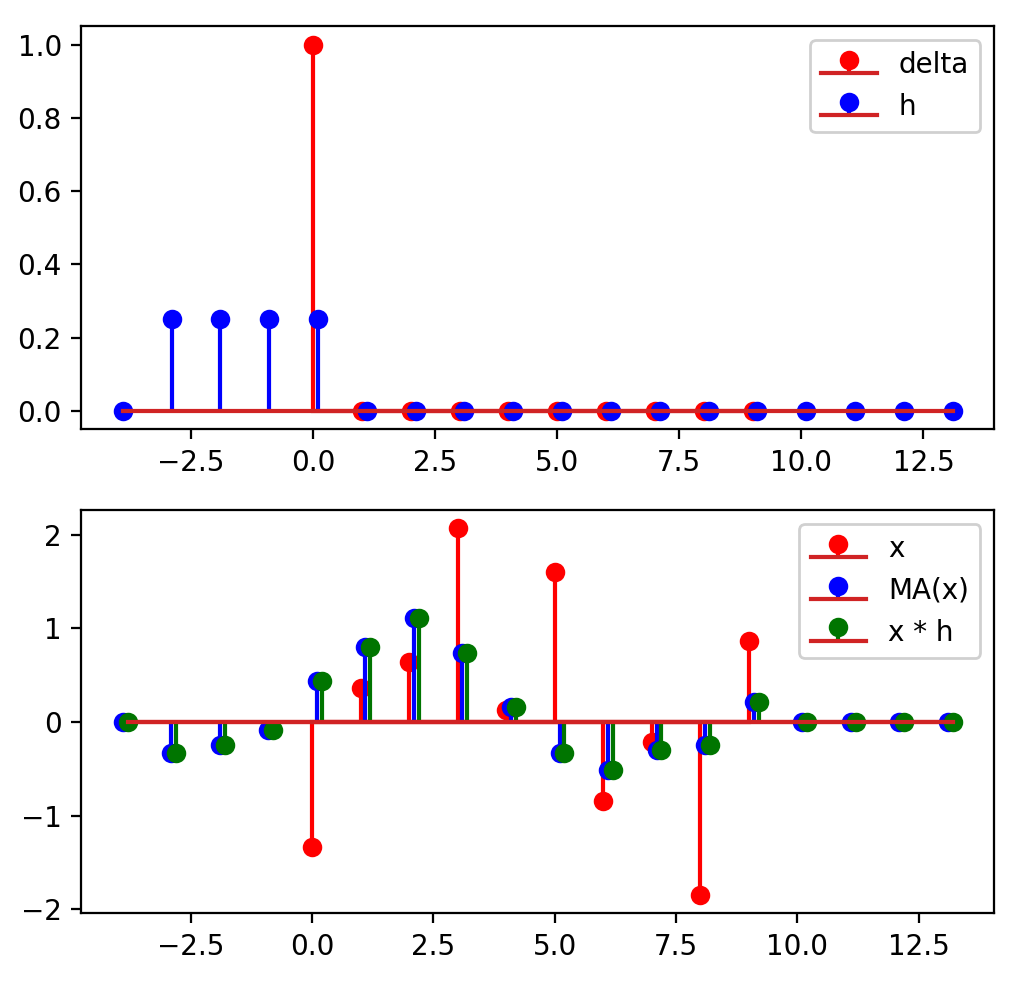
\includegraphics[width=\textwidth]{code/moving_average.png}
    \end{minipage}
    \codecaption{dsv/code/moving_average.py}{Gleitendes Mittel mit L"ange $\ell=4$. Wir vergleichen die direkte Berechnung mit der Berechnung "uber die Faltung}\label{py:moving_average}
\end{listing}

In \Cref{py:moving_average} zeigen wir das Verhalten eines gleitenden Mittelwertes (\emph{moving average}), welches sich durch
\[
y[n] = \frac{1}{\ell} \Sum{k=0}{k=\ell}{x[n-k]}
\]
ergibt.
Man sieht sch"on, dass durch das Mitteln die (in diesem Fall) zuf"allige Eingabe-Sequenz am Ausgang gegl"attet erscheint.
Wichtig bei diesem Beispiel ist die Tatsache, dass wir direkt einsehen, dass Anwendung der direkten Formel f"ur das gleitende Mittel aus eine Eingabe $x[\cdot]$ denselben Effekt hat, wie die Faltung mit $h[\cdot]$, das sich aus der Anwendung der Mittelung auf $\delta[\cdot]$ ergibt.

Es lohnt sich, sich einige Eigenschaften der Faltung zu merken. 
Diese sind:
\begin{itemize}
    \item Bi-Linearit"at: Es gilt $(a_1 x_1[\cdot] + a_2 x_2[\cdot]) \ast h[\cdot] = a_1 (x_1 \ast h)[\cdot] + a_2 (x_2 \ast h)[\cdot]$. 
    Dies ist die \q{normale} Linearit"at in den Eing"angen, die sich aus der Linearit"at des Systems $\mathcal{T}$ ergibt. 
    Es gilt aber auch $(x \ast (a_1 h_1 + a_2 h_2))[\cdot] = a_1 (x \ast h_1)[\cdot] + a_2 (x \ast h_2)[\cdot]$.
    Das hei"st, wenn wir ein System $\mathcal{T} = a_1 \mathcal{T}_1 + a_2 \mathcal{T}_2$ gegeben haben, dann ist die Impulsantwort des Systems $\mathcal{T}$ die gleiche Linearkombination der Impulsantworten $h_1[\cdot]$ und $h_2[\cdot]$ der beiden Systeme $\mathcal{T}_{1,2}$.
    Das hei"st wiederum, dass \gls{lti}-Systeme selbst ein linearer Raum sind!
    Wir sprechen hier von \emph{Bi}-Linearit"at, weil die Faltung eben linear in zwei Argumenten ist.
    \item Die Faltung ist assoziativ: Es gilt also, dass $(x \ast h_1) \ast h_2 = x \ast (h_1 \ast h_2)$. 
    Dies impliziert, dass die Verkettung von zwei \gls{lti}-Systemen wieder ein \gls{lti}-system ergibt, wobei sich die Impulsantwort der Verkettung durch Faltung der beiden Impulsantworten der verketteten Systeme ergibt.
    \item Kommmutativit"at: Es gilt $h_1 \ast h_2 = h_2 \ast h_1$, demnach auch, dass $x \ast (h_1 \ast h_2) = x \ast (h_2 \ast h_1)$.
    Das hei"st erstaunlicherweise, dass man verkettete \gls{lti}-Systeme in ihrer Reihenfolge vertauschen kann, ohne das Eingangs-Ausgangsverhalten des Gesamtsystems zu beeinflussen.
\end{itemize}

\begin{listing}
    \noindent
    \begin{minipage}{0.40\textwidth}
        \strut\vspace*{-\baselineskip}\newline
        \inputminted[firstline=10,lastline=33]{python3}{code/ramp_ma.py}
    \end{minipage}%
    \begin{minipage}{0.59\textwidth}
        \strut\vspace*{-\baselineskip}\newline
        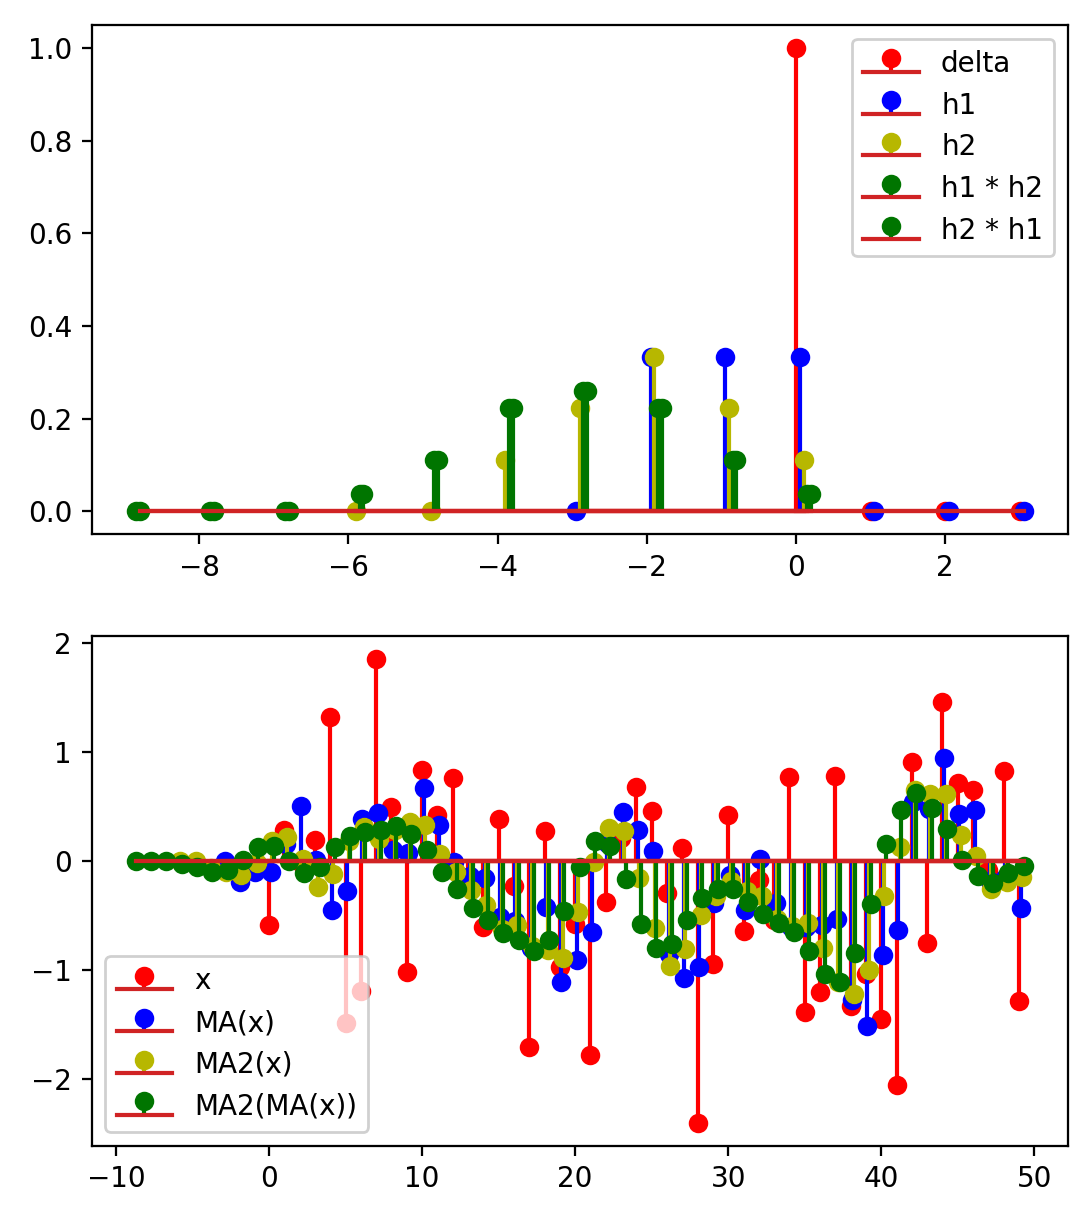
\includegraphics[width=\textwidth]{code/ramp_ma.png}
    \end{minipage}
    \codecaption{dsv/code/ramp_ma.py}{Verkettung von mehreren Moving Averages der L"ange $\ell = 3$.}\label{py:ramp_ma}
\end{listing}
%
In \Cref{py:ramp_ma} untersuchen wir einige der oben genannten Eigenschaften.
Einerseits sehen wir, dass die Impulsantwort von $\texttt{MA}(\texttt{MA2}(\cdot))$ mit der von $\texttt{MA2}(\texttt{MA}(\cdot))$ identisch ist. Wir haben also Kommutativit"at nachgepr"uft.
Wir sehen au"serdem, dass sich die Impulsantwort der Verkettung aus Faltung der einzelnen Impulsantworten ergibt.
Aus dem abgetasteten \q{Rechteck} wird nach nochmaliger Anwendung ein abgetastetes, aber breiteres, \q{Dreieck}, was schlussendlich zu einer abgetasteten, st"uckweise quadratischen, Impulsantwort wird.
Generell kann man das komplette System als eine dreifache Verkettung gleitender Mittel der L"ange $\ell=3$ verstehen.
Au"serdem best"atigt \Cref{py:ramp_ma} bei Vergleich der verschiedenen Ausg"ange, dass wiederholtes Mitteln am Ausgang mit Anzahl der Mittelungen zunehmend \q{glattere} Signale erzeugt.
%
\subsubsection{Eigenschaften von \texorpdfstring{\acrshort{lti}}{LTI}-Systemen}\label{sec:lti_sys:properties}
%
\paragraph{\texorpdfstring{\gls{bibo}}{BIBO}-Stabilit"at}
Wir hatten vorher schon diesen Begriff der Stabili"at eingef"uhrt und formulieren nun eine Bedingung an $h[\cdot]$, die es uns erlaubt auf Stabilit"at zu pr"ufen.
Wir nennen die Eingabe beschr"ankt, falls ein $M_x < \infty$ existiert, sodass
\[
\Abs{x[n]} \leqslant M_x \Text{f"ur alle} n \in \Z
\]
erf"ullt ist.
Dann k"onnen wir mit der Faltungsformel \eqref{eq:lti_sys:conv} berechnen, dass
\[
\Abs{y[n]} 
    = \Abs{\Sum{k\in\Z}{}{x[n] h[n-k]}} 
    \leqslant \Sum{k\in\Z}{}{\Abs{x[n] h[n-k]}} 
    \leqslant M_x \Sum{k\in\Z}{}{\Abs{h[n-k]}} 
\]
gilt.
Damit nun $\Abs{y[n]} < \infty$, muss also gelten, dass
\[
    \Sum{k\in\Z}{}{\Abs{h[n-k]}} < \infty.
\]
Das hei"st, \emph{wenn} $h[\cdot]$ absolut summierbar ist, dann ist das System mit $h[\cdot]$ als Impulsantwort \gls{bibo}-stabil.

Wie ist es um die umgekehrte Schlussfolgerung bestellt?
Impliziert \gls{bibo}-Stabilit"at, dass $h[\cdot]$ absolut summierbar sein muss?
Erinnern wir uns daran, dass man \gls{bibo}-Stabilit"at widerlegen kann, indem man \emph{einen} beschr"ankten Eingang $x[\cdot]$ findet, f"ur welchen der Ausgang $y[\cdot]$ nicht beschr"ankt bleibt.
Nehmen wir an, dass 
\[
\Sum{k\in\Z}{}{\Abs{h[n-k]}} = \infty
\]
und betrachten wir den Eingang
\[
x[n] = \begin{cases}
    \frac{h[-n]^\ast}{\Abs{h[-n]}}, \Text{f"ur} h[n] \neq 0 \\
    0 \Text{sonst.}
\end{cases}
\]
Man sieht, dass $\Abs{x[n]} \leqslant 1$, es ist also beschr"ankt.
Dann berechnen wir einfach den ersten Wert am Ausgang mit \eqref{eq:lti_sys:conv} und der Definition des Einganges $x[\cdot]$, also
\[
y[0] 
    = \Sum{k\in\Z}{}{x[-k] h[k]}
    = \Sum{k\in\Z}{}{
        \frac{\Abs{h[k]}^2}{\Abs{h[k]}}
    }
    = \Sum{k\in\Z}{}{
        \Abs{h[k]}
    }
    = \infty,
\]
wobei das letzte Gleichheitszeichen gilt, weil wir angenommen hatten, dass $h[\cdot]$ nicht absolut summierbar ist.
Man kann also schlussfolgern, dass sich Stabilit"at vollst"andig durch die Impulsantwort $h[\cdot]$ bestimmen l"asst.
Eine tolle Sache!
%
\paragraph{\texorpdfstring{\acrshort{fir}}{FIR} vs. \texorpdfstring{\acrshort{iir}}{IIR}}
%
Gilt f"ur die Impulsantwort $h[\cdot]$, dass
\[
h[n] = 0, \Text{f"ur} n < m, M \leqslant n
\]
f"ur zwei Zahlen $m \leqslant M$, dann bezeichnet man das zugeh"orige System $\mathcal{T}$ als \gls{fir}-System.
Ist obige Bedingung nicht erf"ullt, so nennt man $\mathcal{T}$ ein \gls{iir}-System.
Bei \gls{fir}-Systemen sind f"ur die Berechnung von $y[n]$ nur endlich viele Werte, maximal $M - m$ viele, notwendig.
Das System hat also ein endliches Ged"chtnis der L"ange $M - m$, wobei \gls{iir}-Systeme ein unendlich langes Ged"achtnis haben.
Sobald bei einem \gls{fir}-System $\Abs{h[n]} < \infty$ f"ur alle $n \in \Z$ gilt, ist es auch stabil -- also sind in der Praxis \emph{alle} \gls{fir}-Systeme stabil.

Bei einem \gls{iir}-System ist die Frage nach Stabilit"at nicht so einfach zu beantworten, doch wir werden im Folgenden noch ein Werkzeug kennenlernen, mit welchem dies einfach nachzupr"ufen sein wird.
Au"serdem haben \gls{iir}-Systeme noch das Problem, dass man die Faltungsformel \eqref{eq:lti_sys:conv} nicht nutzen kann, um ein \gls{iir}-System zu \emph{implementieren}.
%
%
\subsubsection{Rekursive \texorpdfstring{\acrshort{iir}}{IIR}-Systeme}
%
%
Um die Notwendigkeit von \eqref{eq:lti_sys:conv} zu umgehen, betrachten wir eine gewisse Klasse von Systemen, deren Ausgang $y[\cdot]$ auch "uber einen alternativen Weg bestimmt werden kann.
Hierzu betrachten wir
\[
y[n] = \frac{1}{n+1}\Sum{k=0}{n}{x[n]},
\]
was ein kumulatives Mittel von $0$ bis $n$ darstellt.
So wie es hier scheint, muss man f"ur die Berechnung von $y[n]$ alle vergangenen Werte von $x[\cdot]$ bereitliegen haben.
Doch mit einer einfachen Umformung findet man, dass
\[
(n+1)y[n] = n y[n-1] + x[n] 
\Leftrightarrow 
y[n] = \frac{n}{n+1} y[n-1] + \frac{1}{n+1} x[n].
\]
Wir k"onnen also alternativ $y[n]$ aus $x[n]$ und $y[n-1]$ berechnen.
Da also $y[n]$ von $y[n-1]$ abh"angt, nennen wir das System \emph{rekursiv}.
Man sieht deutlich, dass diese Umformulierung deutlich macht, dass wir nur $y[n-1]$ im Speicher halten m"ussen und dieses mit einer Art \emph{zeitverz"ogertem Feedback} ausstatten m"ussen.
Hierbei ist nat"urlich die Zeitverz"ogerung essenziell, denn m"ussen wir $y[n]$ in Abh"angigkeit von $y[n]$ berechnen, w"urde uns das vor ein halbwegs unl"osbares Problem stellen.
In \Cref{py:cumulative_sum} sehen wir die beiden unterschiedlichen Implementierungen.
Es ist hier zu beachten, dass \mintinline{python}|y[nn] = np.sum(x[:nn]) / (nn + 1)| immer auf die komplette Vergangenheit von $x[\cdot]$ zugreift und eben \emph{nicht} auf Werte von $y[\cdot]$.

\begin{listing}
    \noindent
    \begin{minipage}{0.49\textwidth}
        \strut\vspace*{-\baselineskip}\newline
        \inputminted[firstline=5,lastline=20]{python3}{code/cumulative_sum.py}
    \end{minipage}%
    \begin{minipage}{0.49\textwidth}
        \strut\vspace*{-\baselineskip}\newline
        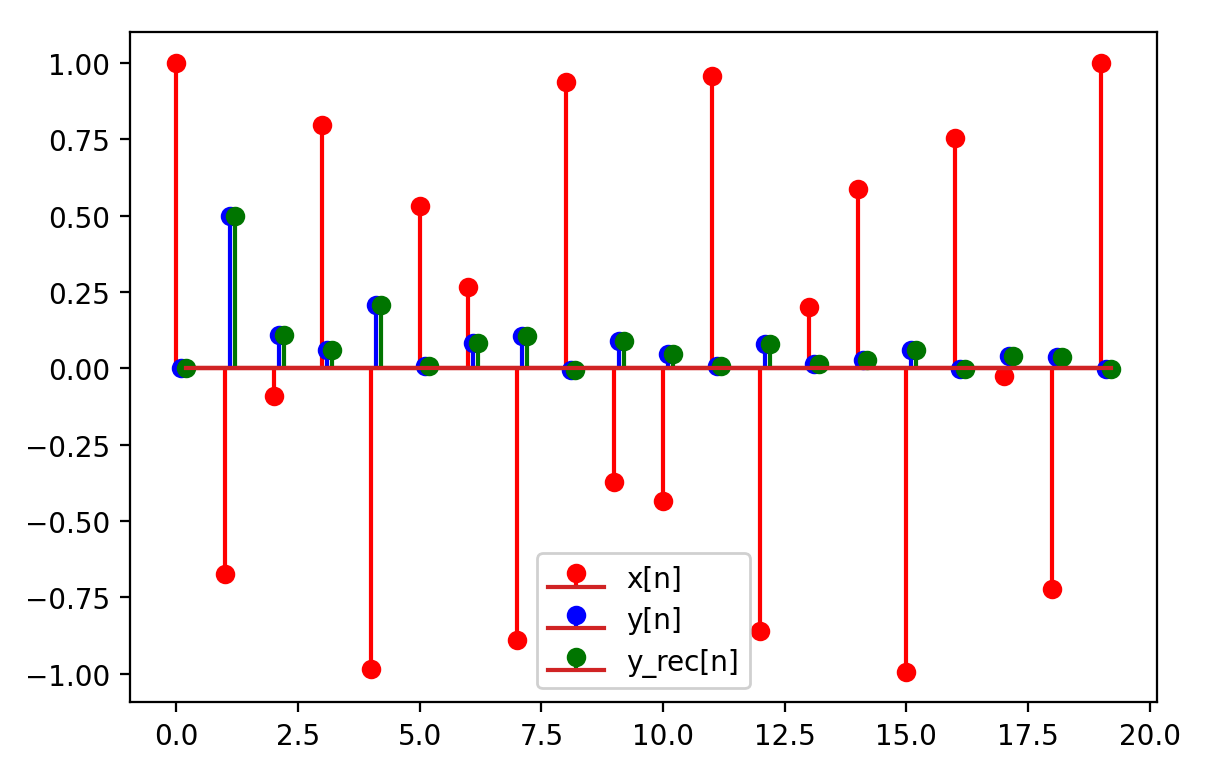
\includegraphics[width=\textwidth]{code/cumulative_sum.png}
    \end{minipage}
    \codecaption{dsv/code/cumulative_sum.py}{Die beiden m"oglichen Implementierungen eines kumulativen Mittelwertes}\label{py:cumulative_sum}
\end{listing}
%
%
F"ur rekursive Systeme entsteht noch das Problem, dass wir beispielsweise f"ur den Beginn der rekursiven Berechnung von $y[n]$ ab einem gewissen $n_0 \in \Z$ den Wert $y[n_0-1]$ kennen m"ussen.
Das hei"st wir ben"otigen einen \emph{Startwert} f"ur die Rekursion.
Dieser beeinflusst auch ma"sgeblich das Verhalten des Systems.

Eine M"oglichkeit, wie man das produktiv ausnutzen kann, ist f"ur die Berechnung der Quadratwurzel einer positiven reellen Zahl $A$.
F"ur die Herleitung definieren wir erst die Funktion $f : \R \rightarrow \R$ via
\[
f(x) = x^2 - A.
\]
Wie man leicht sieht, hat diese Funktion Nullstellen $x_{1,2} = \pm \sqrt{A}$.
Die sogenannte Newton-Iteration~\footnote{\url{https://encyclopediaofmath.org/index.php?title=Newton_method}} berechnet iterativ via
\[
y[n] = y[n-1] - \frac{f(y[n-1])}{f^\prime(y[n-1])}
\]
eine Nullstelle der Funktion $f$.
Setzen wir unsere Funktion ein und definieren $x[\cdot] = A u[\cdot]$, dann erhalten wir
\[
y[n] = \frac 12 \left(
    y[n-1] + \frac{x[n]}{y[n-1]}.
\right)
\]
Nutzen wir einen geeigneten Startwert, beispielsweise $y[-1] = 1$, so erhalten wir eine \emph{sehr schnell} konvergierende Folge von $y[n]$.

\begin{listing}
    \noindent
    \begin{minipage}{0.49\textwidth}
        \strut\vspace*{-\baselineskip}\newline
        \inputminted[firstline=5,lastline=15]{python3}{code/square_root.py}
    \end{minipage}%
    \begin{minipage}{0.49\textwidth}
        \strut\vspace*{-\baselineskip}\newline
        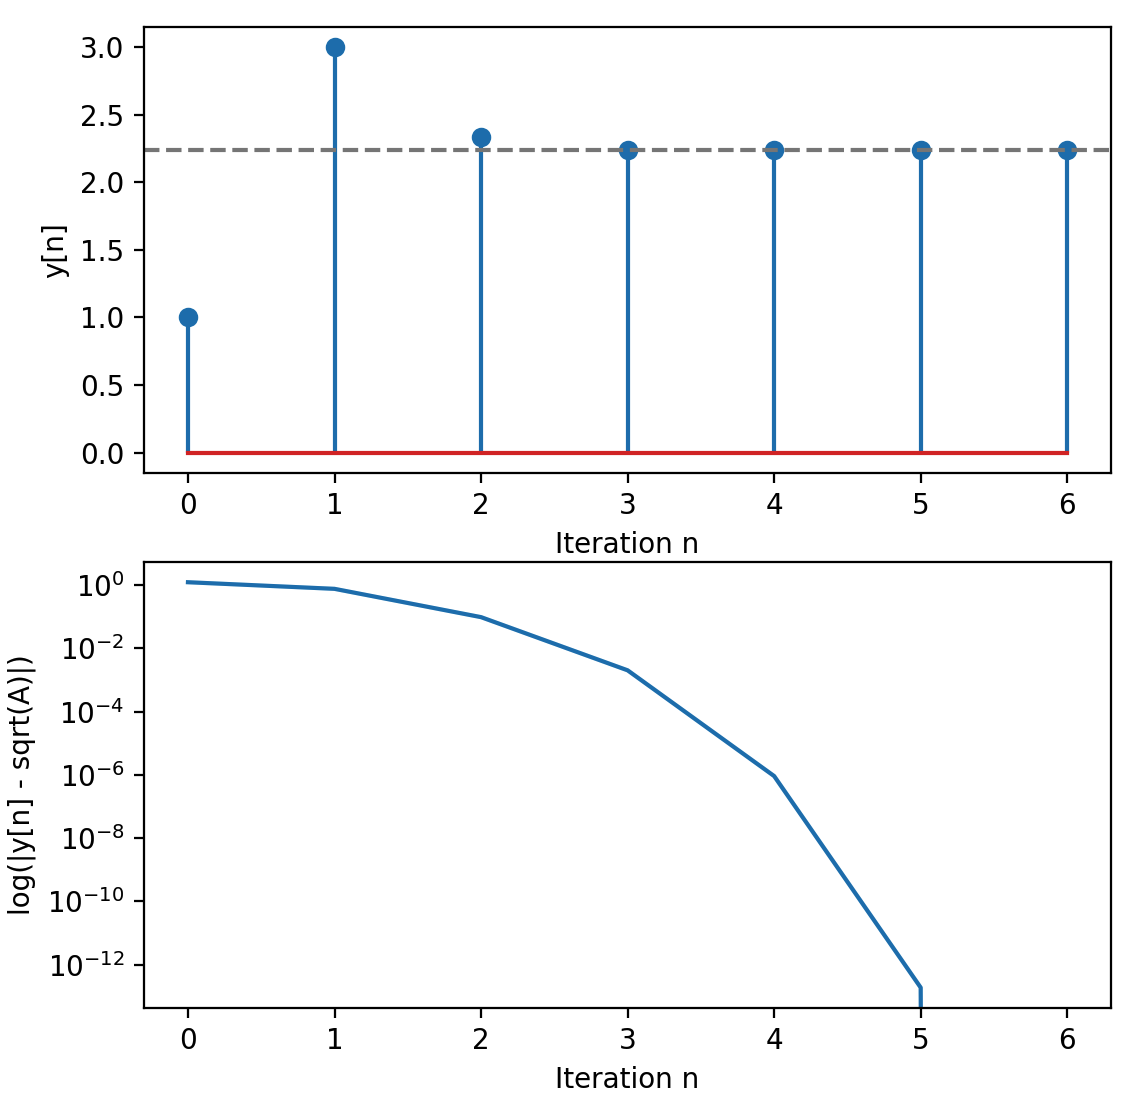
\includegraphics[width=\textwidth]{code/square_root.png}
    \end{minipage}
    \codecaption{dsv/code/square_root.py}{Iteratives Verfahren zur Berechnung von $\sqrt{A}$}\label{py:square_root}
\end{listing}
%
%
Die Folge konvergiert so schnell, dass bereits nach $5$ Iterationen der Fehler an der endlichen Genauigkeit von Gleitkommaarithmetik kratzt.
Es ist auch darauf hinzuweisen, dass das System nur sehr einfache arithmetische Operationen benutzt, um die numerisch nicht ganz triviale Berechnung von $\sqrt{A}$ beliebig genau und sehr schnell zu approximieren.

Abschlie"send ist noch anzumerken, dass man rekursive Systeme auch \q{l"osen} kann, siehe \cite[Kap.~2.4.3]{proakis2013}, indem man aus der rekursiven Vorschrift eine explizite entwickelt. 
Die dort entwickelte Theorie erinnert der L"osung von Differenzialgleichungen nach Funktionen, nur werden stattdessen Differenzengleichungen nach diskreten Folgen gel"ost.
%
%
\subsubsection{Approximation von \texorpdfstring{\acrshort{iir}}{IIR}-Systemen durch \texorpdfstring{\acrshort{fir}}{FIR}-Systeme}
Um die Faltungsformel doch anwenden zu k"onnen, kann man f"ur ein \emph{stabiles} \gls{iir}-System mit Impulsantwort $h[\cdot]$ eine \gls{fir}-Approximation finden.
Ein weiterer Vorteil ergibt sich dann, dass auch dieses resultierende System stabil sein muss.
F"ur $n_{\rm low} < n_{\rm hgh}$ definieren wir
\[
h_{\rm FIR}[n] = \begin{cases}
    h[n], \Text{falls} n_{\rm low} \leqslant n \leqslant n_{\rm hgh}, \\
    0 \Text{sonst.}
\end{cases}
\]
Da aus der Stabilit"at von dem System mit Impulsantwort $h[\cdot]$ folgt, dass
\[
    \lim\limits_{k \rightarrow \infty} 
        \Sum{n = k}{\infty}{
            \left(\Abs{h[n]} + \Abs{h[-n]}\right)
        } = 0,
\]
da sonst
\[
    \Sum{n \in \Z}{\infty}{\Abs{h[n]}}
\]
nicht endlich sein k"onnte.
Das hei"st, dass die Werte der Impulsantwort $h[\cdot]$ gegen $0$ konvergieren m"ussen und deshalb kann man $n_{\rm low} < n_{\rm hgh}$ so w"ahlen, dass der Unterschied zwischen $h[\cdot]$ und $h_{\rm FIR}[\cdot]$ beliebig klein wird.

Je nachdem wie schnell $h[\cdot]$ gegen $0$ konvergiert, ben"otigen wir mehr oder von $0$ verschiedene Eintr"age in $h_{\rm FIR}$, was sich auf den Implementierungsaufwand auswirkt.

Ein Beispiel f"ur einen exponentiellen Mittelwert-Filter findet man in \Cref{py:exp_mean}.
Man sieht, dass f"ur $\alpha=0.5$ der Abschneidefehler deutlicher zutage tritt, da die Faltung mit $h_{\rm FIR}[\cdot]$ in diesem Fall ein deutlich schlechteres Ergebnis liefert als im Falle von $\alpha=0.1$.
Dies liegt eben daran, dass bei $\alpha=0.1$ der \gls{iir}-Filter \emph{effektiv} ein \gls{fir}-Filter wird.
Wir wollen aber darauf hinweisen, dass es eine ganz eigene Theorie f"ur die Approximation von Filtern durch andere Filter gibt, die wir hier nicht einmal anrei"sen wollen.

\begin{listing}
    \noindent
    \begin{minipage}{0.49\textwidth}
        \strut\vspace*{-\baselineskip}\newline
        \inputminted[firstline=5,lastline=33]{python3}{code/exp_mean.py}
    \end{minipage}%
    \begin{minipage}{0.49\textwidth}
        \strut\vspace*{-\baselineskip}\newline
        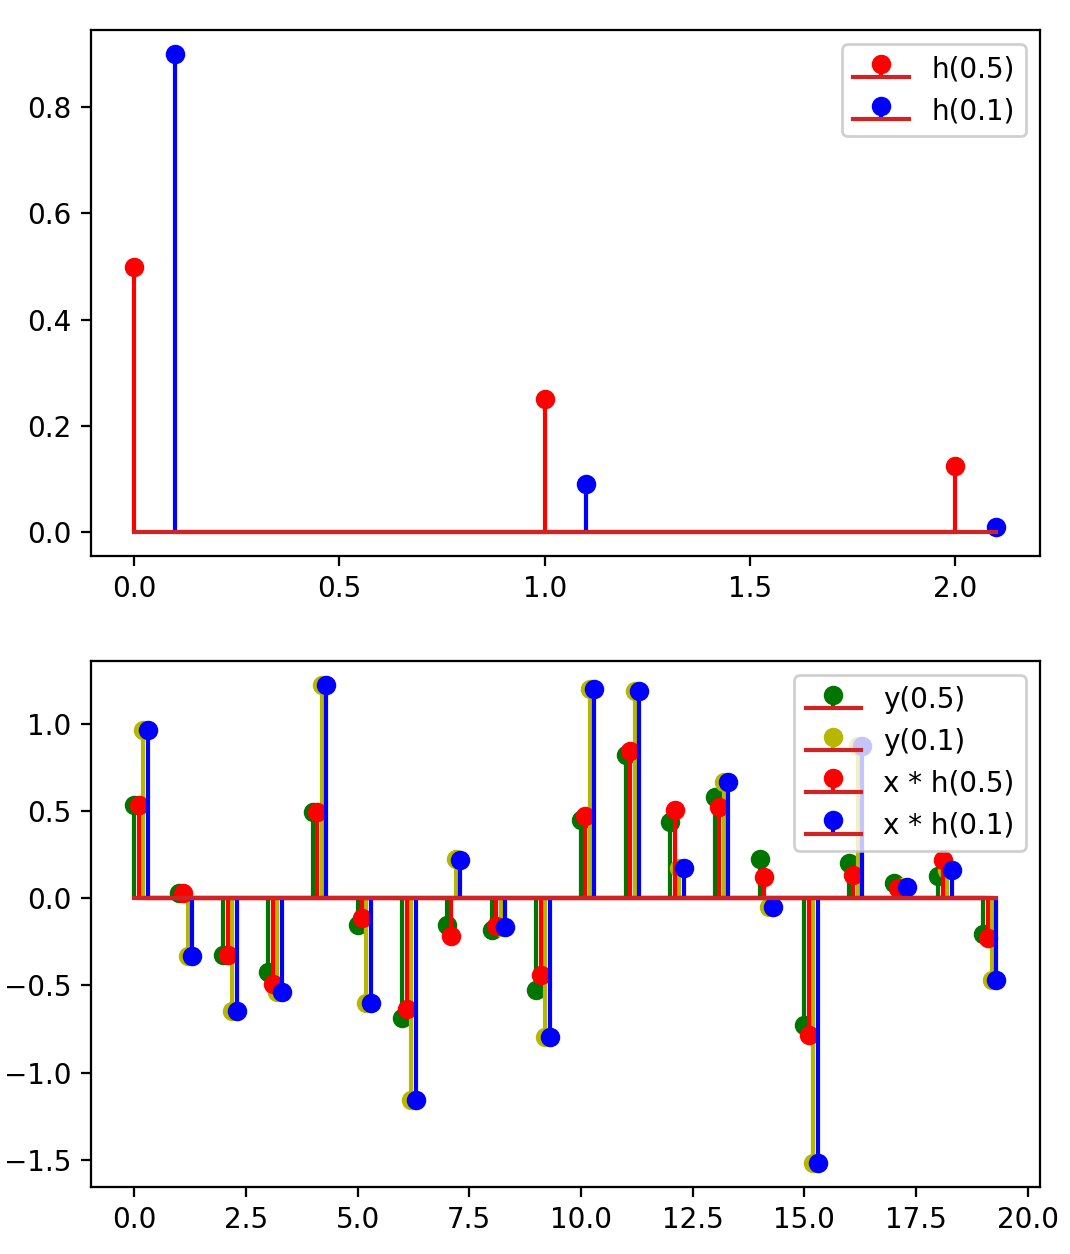
\includegraphics[width=\textwidth]{code/exp_mean.png}
    \end{minipage}
    \codecaption{dsv/code/exp_mean.py}{Approximation eines exponentiellen Mittelwertes, also einem \gls{iir}-System, durch ein \gls{fir}-System}\label{py:exp_mean}
\end{listing}